\documentclass[11pt]{article} % use larger type; default would be 10pt

\usepackage[utf8]{inputenc} % set input encoding (not needed with XeLaTeX)
\usepackage{adjustbox}   
%%% Examples of Article customizations
% These packages are optional, depending whether you want the features they provide.
% See the LaTeX Companion or other references for full information.
  
%%%%%%%%%%%%%%%%%%%%%%%%%%formatting cells colors
\usepackage[table,x11names,dvipsnames]{xcolor}
 \usepackage{collcell}
 \usepackage{array}
 \usepackage{tikz}
  \usepackage{pgfkeys}
 \usepackage{graphicx}
 \usepackage{amsmath,amssymb}

 \pgfkeys{/heat/.is family, /heat,
      Max colour/.initial = Green4,
      Min colour/.initial = Red1,
      max colour/.initial = SpringGreen3,
      mid colour/.initial = white,
      min colour/.initial = Yellow1,
      text colour/.initial = black,
      Min color/.style = {Min colour=#1},% for our friends who can't spell
      Max color/.style = {Max colour=#1},
      min color/.style = {min colour=#1},
      mid color/.style = {mid colour=#1},
      max color/.style = {max colour=#1},
      text color/.style = {text colour=#1},
      min/.initial = -1,
      mid/.initial = 0,
      max/.initial = 1,
      slider/.code={%
         \tikz{\shade[left color=\HVal{min colour},%
                      right color=\HVal{max colour}]%
            (current page.south west) rectangle ++(#1,12pt);
         }%
      }%
  }
  \newcommand\Heatset[1]{\pgfkeys{/heat, #1}}
  \newcommand\HVal[1]{\pgfkeysvalueof{/heat/#1}}

  \newcolumntype{H}{>{\collectcell\Heat}r<{\endcollectcell}}
  \newcommand\Heat[1]{% \Heat{number in the interval [min, max] }
    \if\relax\detokenize{#1}\relax% empty cell
    \else%
      \pgfmathparse{int(100*(#1-\HVal{min})/(\HVal{max}-\HVal{min}))}% map number to [0,100]
      \ifnum\pgfmathresult>100% too big
        \edef\HeatCell{\noexpand\cellcolor{\HVal{Max colour}}}%
      \else\ifnum\pgfmathresult<0% too small
          \edef\HeatCell{\noexpand\cellcolor{\HVal{Min colour}}}%
      \else\ifnum\pgfmathresult<50% between min and mid
	      \pgfmathparse{int(2*\pgfmathresult)}% map number to [0,100]
		  \edef\HeatCell{\noexpand\cellcolor{\HVal{mid colour}!\pgfmathresult!\HVal{min colour}}}%
		\else% between min and max
	      \pgfmathparse{int(2*(\pgfmathresult-50))}% map number to [0,100]
          \edef\HeatCell{\noexpand\cellcolor{\HVal{max colour}!\pgfmathresult!\HVal{mid colour}}}%
        \fi%
        \fi%
      \fi%
      \HeatCell\textcolor{\HVal{text colour}}{$#1$}%
    \fi%
  }

 \pgfkeys{/heatsec/.is family, /heatsec,
	Max colour/.initial = Green4,
	Min colour/.initial = Red1,
	max colour/.initial = SpringGreen3,
	mid colour/.initial = white,
	min colour/.initial = Yellow1,
	text colour/.initial = black,
	Min color/.style = {Min colour=#1},% for our friends who can't spell
	Max color/.style = {Max colour=#1},
	min color/.style = {min colour=#1},
	mid color/.style = {mid colour=#1},
	max color/.style = {max colour=#1},
	text color/.style = {text colour=#1},
	min/.initial = -1,
	mid/.initial = 0,
	max/.initial = 1,
	slider/.code={%
		\tikz{\shade[left color=\HVal{min colour},%
			right color=\HVal{max colour}]%
			(current page.south west) rectangle ++(#1,12pt);
		}%
	}%
}
\newcommand\HeatSecset[1]{\pgfkeys{/heatsec, #1}}
\newcommand\HSVal[1]{\pgfkeysvalueof{/heatsec/#1}}

\colorlet{BadCol}{Burlywood1!70!red}


\newcolumntype{S}{>{\collectcell\HeatSec}r<{\endcollectcell}}
\newcommand\HeatSec[1]{% \Heat{number in the interval [min, max] }
	\if\relax\detokenize{#1}\relax% empty cell
	\else%
	\pgfmathparse{int(100*(#1-\HSVal{min})/(\HSVal{max}-\HSVal{min}))}% map number to [0,100]
	\ifnum\pgfmathresult>100% too big
	\edef\HeatCell{\noexpand\cellcolor{\HSVal{Max colour}}}%
	\else\ifnum\pgfmathresult<0% too small
	\edef\HeatCell{\noexpand\cellcolor{\HSVal{Min colour}}}%
	\else\ifnum\pgfmathresult<50% between min and mid
	\pgfmathparse{int(2*\pgfmathresult)}% map number to [0,100]
	\edef\HeatCell{\noexpand\cellcolor{\HSVal{mid colour}!\pgfmathresult!\HSVal{min colour}}}%
	\else% between min and max
	\pgfmathparse{int(2*(\pgfmathresult-50))}% map number to [0,100]
	\edef\HeatCell{\noexpand\cellcolor{\HSVal{max colour}!\pgfmathresult!\HSVal{mid colour}}}%
	\fi%
	\fi%
	\fi%
	\HeatCell\textcolor{\HSVal{text colour}}{$#1$}%
	\fi%
}

%%% PAGE DIMENSIONS
\usepackage{geometry} % to change the page dimensions
\geometry{a4paper} % or letterpaper (US) or a5paper or....
% \geometry{margin=2in} % for example, change the margins to 2 inches all round
% \geometry{landscape} % set up the page for landscape
%   read geometry.pdf for detailed page layout information
\usepackage{multicol}
\usepackage{booktabs}
\usepackage{todonotes}
\title{Supplementary materials}
%\author{}
%\date{} % Activate to display a given date or no date (if empty),
         % otherwise the current date is printed 
\newcommand{\Software}[1]{\texttt{#1}}
\newcommand{\OurTool}{\Software{IPANEMAP}}
\newcommand{\Start}{s}
\newcommand{\End}{e}

\newcommand{\yp}[1]{{\todo[color=blue!30]{\sf Yann: #1}}}

\begin{document}
\maketitle

\section{ Cordero~\emph{et al} dataset}
\subsection{Structure prediction ordered by RNA}

 \Heatset{min=0.4,  
	max=1,   
	max colour=Aquamarine3, % colour at maximum
	min colour=BadCol,      % colour at minimum
	Min colour=BadCol, % colour for values below min
	Max colour=Aquamarine3   % colour for values above max
}
\begin{table}[h]
\centering
\begin{adjustbox}{max width=1\textwidth}
 \begin{tabular}{lHHHHHHHHHHHHHHHHHHHHH}
 &\multicolumn{8}{l}{ \OurTool{}} & \multicolumn{4}{l}{ RNAfold MFE} & \multicolumn{4}{l}{RNAfold MEA} \\
% & \multicolumn{3}{l}{ GM }  & \multicolumn{3}{l}{ GM } & \multicolumn{3}{l}{ GM }& \multicolumn{3}{l}{ GM }  & \multicolumn{3}{l}{ GM } & \multicolumn{3}{l}{ GM } &\multicolumn{3}{l}{ GM }\\
\toprule
\textbf{RNA }& \multicolumn{1}{l}{(-)} & \multicolumn{1}{l}{CMCT} & \multicolumn{1}{l}{NMIA} & \multicolumn{1}{l}{DMS} & \multicolumn{1}{l}{DMS+NMIA} & \multicolumn{1}{l}{DMS+CMCT}& \multicolumn{1}{l}{NMIA+CMCT}	 & \multicolumn{1}{l}{DMS+NMIA+CMCT} & \multicolumn{1}{l}{(-)}& \multicolumn{1}{l}{DMS }& \multicolumn{1}{l}{CMCT} &\multicolumn{1}{l}{ NMIA}& \multicolumn{1}{l}{(-)} & \multicolumn{1}{l}{DMS} & \multicolumn{1}{l}{CMCT} & \multicolumn{1}{l}{NMIA}\\
\midrule
5SRNA,E.Coli		&	0.25	&	0.238	&	0.247	&	0.244	&	0.247	&	0.247	&	0.254	&	0.241	&	0.241	&	0.686	&	0.254	&	0.686	&	0.241	&	0.686	&	0.269	&	0.686	\\
glycineriboswitch,F.nucleatum		&	0.568	&	0.627	&	0.868	&	0.952	&	0.868	&	0.658	&	0.868	&	0.868	&	0.306	&	0.313	&	0.395	&	0.313	&	0.593	&	0.593	&	0.693	&	0.6	\\
cidGMPriboswitch,V.Cholerae		&	0.654	&	0.77	&	0.654	&	0.77	&	0.654	&	0.77	&	0.654	&	0.77	&	0.77	&	0.77	&	0.667	&	0.77	&	0.77	&	0.72	&	0.667	&	0.77	\\
P4P6domain		&	0.864	&	0.856	&	0.881	&	0.864	&	0.864	&	0.856	&	0.864	&	0.856	&	0.837	&	0.808	&	0.773	&	0.714	&	0.845	&	0.808	&	0.781	&	0.722	\\
adenineriboswitch,add		&	1	&	0.956	&	1	&	0.977	&	1	&	0.956	&	1	&	1	&	1	&	0.333	&	0.41	&	1	&	1	&	0.333	&	0.356	&	0.306	\\
tRNAphenylalanineyeast		&	0.286	&	0.746	&	0.976	&	0.746	&	0.976	&	0.746	&	0.976	&	0.976	&	0.976	&	0.976	&	0.976	&	0.976	&	0.334	&	0.976	&	0.976	&	0.976	\\

\midrule
Average&0.604&0.7&0.77&0.76&0.77&0.705&0.77&0.785&0.69&0.65&0.58&0.74&0.63&0.69&0.62&0.68\\
\bottomrule
\end{tabular}
\end{adjustbox}
\caption{ GM of the predicted structures with \OurTool{} compared to RNAfold MFE and MEA resulting structures}
%( ref. $supplementary\_data/benchmark\_6RNAs$)}
\end{table}
\subsection{Reproducibility}
\begin{table}[h]
\centering
\begin{adjustbox}{max width=1\textwidth}
 \begin{tabular}{lHHHHHHHHHHHHHHHHHHHHH}
 &\multicolumn{3}{l}{ NMIA} & \multicolumn{3}{l}{ DMS} & \multicolumn{3}{l}{CMCT} &\multicolumn{3}{l}{ NMIA+DMS} & \multicolumn{3}{l}{ NMIA+CMCT} & \multicolumn{3}{l}{DMS+CMCT}& \multicolumn{3}{l}{NMIA+DMS+CMCT} \\
% & \multicolumn{3}{l}{ GM }  & \multicolumn{3}{l}{ GM } & \multicolumn{3}{l}{ GM }& \multicolumn{3}{l}{ GM }  & \multicolumn{3}{l}{ GM } & \multicolumn{3}{l}{ GM } &\multicolumn{3}{l}{ GM }\\
\toprule
\textbf{RNA }& \multicolumn{1}{l}{run 1} & \multicolumn{1}{l}{run 2} & \multicolumn{1}{l}{run 3} & \multicolumn{1}{l}{run 1} & \multicolumn{1}{l}{run 2} & \multicolumn{1}{l}{run 3}& \multicolumn{1}{l}{run 1} & \multicolumn{1}{l}{run 2} & \multicolumn{1}{l}{run 3} & \multicolumn{1}{l}{run 1} & \multicolumn{1}{l}{run 2} & \multicolumn{1}{l}{run 3}& \multicolumn{1}{l}{run 1} & \multicolumn{1}{l}{run 2} & \multicolumn{1}{l}{run 3} & \multicolumn{1}{l}{run 1} & \multicolumn{1}{l}{run 2} & \multicolumn{1}{l}{run 3}& \multicolumn{1}{l}{run 1} & \multicolumn{1}{l}{run 2} & \multicolumn{1}{l}{run 3}\\
\midrule
5SRNA,E.Coli	&	0.247	&	0.25	&	0.247	&	0.254	&	0.244	&	0.244	&	0.238	&	0.238	&	0.238	&	0.247	&	0.244	&	0.247	&	0.257	&	0.238	&	0.238	&	0.247	&	0.247	&	0.244	&	0.241	&	0.241	&	0.241	\\
glycineriboswitch,F.nucleatum	&	0.868	&	0.868	&	0.868	&	0.952	&	0.952	&	0.952	&	0.868	&	0.634	&	0.627	&	0.868	&	0.868	&	0.868	&	0.868	&	0.868	&	0.868	&	0.667	&	0.658	&	0.658	&	0.868	&	0.868	&	0.868	\\
cidGMPriboswitch,V.Cholerae	&	0.631	&	0.631	&	0.631	&	0.77	&	0.77	&	0.77	&	0.667	&	0.77	&	0.77	&	0.631	&	0.631	&	0.756	&	0.77	&	0.77	&	0.77	&	0.77	&	0.77	&	0.77	&	0.77	&	0.77	&	0.77	\\
P4P6domain	&	0.864	&	0.881	&	0.881	&	0.864	&	0.864	&	0.856	&	0.856	&	0.856	&	0.856	&	0.864	&	0.864	&	0.864	&	0.864	&	0.864	&	0.864	&	0.856	&	0.856	&	0.856	&	0.856	&	0.856	&	0.856	\\
adenineriboswitch,ad	&	1	&	1	&	1	&	0.956	&	0.956	&	0.956	&	1	&	0.956	&	0.956	&	1	&	1	&	1	&	1	&	1	&	1	&	0.956	&	0.956	&	0.956	&	1	&	1	&	1	\\
tRNAphenylalanineyeast	&	0.953	&	0.953	&	0.976	&	0.976	&	0.746	&	0.976	&	0.746	&	0.746	&	0.746	&	0.976	&	0.976	&	0.976	&	0.976	&	0.976	&	0.97	&	0.746	&	0.746	&	0.746	&	0.746	&	0.976	&	0.976	\\

\bottomrule
\end{tabular}
\end{adjustbox}
\caption{ GM of the predicted structures with \OurTool{} over 3 runs, in the presence of 1,2 and 3 sources of probing data}
%( ref. $supplementary\_data/benchmark\_6RNAs$)
\end{table}



%\section{IPANEMAP Vs Rsample}
\section{Hadjin ~\emph{et al} dataset}

  \Heatset{min=0.4,  
	max=1,   
	max colour=Aquamarine3, % colour at maximum
	min colour=BadCol,      % colour at minimum
	Min colour=BadCol, % colour for values below min
	Max colour=Aquamarine3   % colour for values above max
}
\begin{table}
\begin{adjustbox}{max width=\textwidth,max totalheight=\textheight,keepaspectratio}
\begin{tabular}{llllHllH}
\toprule
\textbf{RNA} & Length &  \multicolumn{3}{l}{\Software{Rsample}} &  \multicolumn{3}{l}{\Software{IPANEMAP}} \\
\midrule
	&		&	Sensitivity	&	PPV	&	\multicolumn1c{GM}	&	Sensitivity	&	PPV	&	\multicolumn1c{GM}	\\
A	&	34	&	0.625	&	1	&	0.791	&	0.625	&	1	&	0.791	\\
B	&	530	&	0.6622	&	0.6203	&	0.641	&	0.8986	&	0.8062	&	0.851	\\
C	&	301	&	0.03	&	0.0313	&	0.031	&	0.6	&	0.6	&	0.6	\\
D	&	214	&	0.6349	&	0.6667	&	0.651	&	0.7302	&	0.8519	&	0.789	\\
E	&	500	&	0.6382	&	0.7823	&	0.707	&	0.5263	&	0.5517	&	0.539	\\
F	&	47	&	0.4	&	0.75	&	0.548	&	0.6	&	0.75	&	0.671	\\
G	&	118	&	0.7179	&	0.8	&	0.758	&	0.7692	&	0.8333	&	0.801	\\
H	&	76	&	0.4762	&	0.5556	&	0.514	&	0.7619	&	0.7619	&	0.762	\\
I	&	155	&	0.6786	&	0.8261	&	0.749	&	0.9821	&	0.9821	&	0.982	\\
J	&	79	&	0.7727	&	0.85	&	0.81	&	0.9545	&	0.875	&	0.914	\\
K	&	71	&	1	&	1	&	1	&	1	&	0.9545	&	0.977	\\
L	&	66	&	0.5625	&	0.6923	&	0.624	&	0.625	&	0.7143	&	0.668	\\
M	&	79	&	0.6538	&	0.8095	&	0.727	&	0.6538	&	0.68	&	0.667	\\
N	&	120	&	0.2857	&	0.2632	&	0.274	&	0.9714	&	0.9189	&	0.945	\\
O	&	97	&	0.9286	&	0.9286	&	0.929	&	0.9286	&	0.8966	&	0.912	\\
P	&	511	&	0.9328	&	0.7762	&	0.851	&	0.8908	&	0.7681	&	0.827	\\
Q	&	401	&	0.5826	&	0.5583	&	0.57	&	0.7304	&	0.75	&	0.74	\\
R	&	425	&	0.8397	&	0.8271	&	0.833	&	0.9084	&	0.8815	&	0.895	\\
S	&	336	&	0.5481	&	0.6129	&	0.58	&	0.8077	&	0.866	&	0.836	\\
T	&	473	&	0.7986	&	0.7143	&	0.755	&	0.8819	&	0.8194	&	0.85	\\
U	&	412	&	0.5379	&	0.6174	&	0.576	&	0.75	&	0.8462	&	0.797	\\
V	&	75	&	0.619	&	0.6842	&	0.651	&	0.619	&	0.5652	&	0.591	\\
W	&	174	&	0.8095	&	0.8644	&	0.836	&	0.8095	&	0.9808	&	0.891	\\
X	&	154	&	0.875	&	0.913	&	0.894	&	0.875	&	0.913	&	0.894	\\

\bottomrule
\end{tabular}
\end{adjustbox}
\caption{\OurTool~ prediction performance compared to \Software{Rsample} tool}
\end{table}

 \begin{table}[h]
\centering
\begin{adjustbox}{max width=1\textwidth}
 \begin{tabular}{@{}ll@{}}
 \toprule
Rna ID & Description\\
 \midrule
A	&	PreQ1riboswitchBsubtilis\\
B	&	5domainof16SrRNAEcoli\\
C	&	SignalrecognitonparticleRNAhuman\\
D	&	GroupIintronAzoarcussp\\
E	&	HIV15primepseudoknotdomain\\
F	&	Telomerasepseudoknothuman\\
G	&	SAMIriboswitchTtengcongensis\\
H	&	tRNApheEcoli\\
I	&	P546domainbI3groupIintron\\
J	&	TPPriboswitchEcoli\\
K	&	AdenineriboswitchVvulnificus\\
L	&	FluorideriboswitchPsyringae\\
M	&	SARScoronaviruspseudoknot\\
N	&	5SrRNAEcoli\\
O	&	cyclicdiGMPriboswitchVcholerae\\
P	&	5domainof23SrRNAEcoli\\
Q	&	RNasePBsubtilis\\
R	&	GroupIIntronTthermophila\\
S	&	HepatitisCvirusIRESdomain\\
T	&	5domainof16SrRNAHvolcanii\\
U	&	GroupIIintronOiheyensis\\
V	&	tRNAaspyeast\\
W	&	LysineriboswitchTmaritime\\
X	&	MBoxriboswitchBsubtilis\\
\bottomrule
\end{tabular}
\end{adjustbox}
\caption{24 RNAs from Hadjin \emph{ et al.} dataset.}
\label{clyu}


\end{table}
%  \Heatset{min=0,  
%	max=1,   
%	max colour=Aquamarine3, % colour at maximum
%	min colour=BadCol,      % colour at minimum
%	Min colour=BadCol, % colour for values below min
%	Max colour=Aquamarine3   % colour for values above max
%}

\begin{table}
\begin{adjustbox}{max width=\textwidth,max totalheight=\textheight,keepaspectratio}
\begin{tabular}{llHHHHHHHHHHHlHH}
\toprule
\textbf{RNA} & Length &  \multicolumn1c{Run1} &\multicolumn1c{Run2}&\multicolumn1c{Run3}&\multicolumn1c{Run4}&\multicolumn1c{Run5}&\multicolumn1c{Run6}&\multicolumn1c{Run7}&\multicolumn1c{Run8}&\multicolumn1c{Run9}&\multicolumn1c{Run10}& \multicolumn1c{Average}& \multicolumn1c{Sd}&\multicolumn1c{\textbf{MFE-RNAfold}} & \multicolumn1c{\textbf{MEA-RNAfold}}\\
\midrule

A	&	34	&	0.791	&	0.791	&	0.791	&		0.791	&	0.791	&	0.791	&	0.791	&	0.791	&	0.791	&	0.722	&	0.7841	&	0.0207	&	0.791	&	0.791	\\
B	&	530	&	0.851	&	0.851	&	0.851	&		0.851	&	0.851	&	0.851	&	0.851	&	0.851	&	0.851	&	0.851	&	0.851	&	0	&	0.851	&	0.849	\\
C	&	301	&	0.6	&	0.6	&	0.6	&		0.6	&	0.6	&	0.6	&	0.6	&	0.6	&	0.6	&	0.6	&	0.6	&	0	&	0.6	&	0.597	\\
D	&	214	&	0.789	&	0.789	&	0.789	&		0.781	&	0.781	&	0.781	&	0.781	&	0.781	&	0.781	&	0.781	&	0.7834	&	0.0037	&	0.768	&	0.761	\\
E	&	500	&	0.539	&	0.539	&	0.539	&		0.539	&	0.539	&	0.539	&	0.539	&	0.535	&	0.541	&	0.515	&	0.5364	&	0.0073	&	0.562	&	0.524	\\
F	&	47	&	0.671	&	0.671	&	0.671	&		0.671	&	0.671	&	0.671	&	0.671	&	0.671	&	0.671	&	0.671	&	0.671	&	0	&	0.671	&	0.671	\\
G	&	118	&	0.801	&	0.801	&	0.801	&		0.801	&	0.801	&	0.801	&	0.801	&	0.801	&	0.801	&	0.801	&	0.801	&	0	&	0.892	&	0.879	\\
H	&	76	&	1	&	1	&	1	&		1	&	1	&	1	&	1	&	0.762	&	0.762	&	0.781	&	0.9305	&	0.1063	&	1	&	1	\\
I	&	155	&	0.982	&	0.982	&	0.982	&		0.982	&	0.982	&	0.982	&	0.982	&	0.982	&	0.982	&	0.964	&	0.9802	&	0.0054	&	0.964	&	0.982	\\
J	&	79	&	0.914	&	0.914	&	0.914	&		0.914	&	0.914	&	0.914	&	0.914	&	0.914	&	0.597	&	0.889	&	0.8798	&	0.0946	&	0.914	&	0.914	\\
K	&	71	&	1	&	1	&	1	&		1	&	1	&	1	&	1	&	0.977	&	0.977	&	0.977	&	0.9931	&	0.0105	&	1	&	1	\\
L	&	66	&	0.668	&	0.668	&	0.668	&		0.668	&	0.668	&	0.668	&	0.668	&	0.668	&	0.668	&	0.668	&	0.668	&	0	&	0.668	&	0.668	\\
M	&	79	&	0.706	&	0.706	&	0.706	&		0.706	&	0.706	&	0.706	&	0.721	&	0.721	&	0.667	&	0.745	&	0.709	&	0.0184	&	0.692	&	0.692	\\
N	&	120	&	0.945	&	0.945	&	0.945	&		0.945	&	0.945	&	0.945	&	0.812	&	0.812	&	0.812	&	0.823	&	0.8929	&	0.064	&	0.945	&	0.914	\\
O	&	97	&	0.912	&	0.912	&	0.912	&		0.912	&	0.912	&	0.912	&	0.912	&	0.912	&	0.929	&	0.929	&	0.9154	&	0.0068	&	0.948	&	0.948	\\
P	&	511	&	0.824	&	0.824	&	0.824	&		0.821	&	0.821	&	0.818	&	0.818	&	0.833	&	0.83	&	0.827	&	0.824	&	0.0046	&	0.831	&	0.828	\\
Q	&	401	&	0.74	&	0.74	&	0.74	&		0.74	&	0.74	&	0.74	&	0.74	&	0.74	&	0.74	&	0.74	&	0.74	&	0	&	0.813	&	0.75	\\
R	&	425	&	0.895	&	0.895	&	0.895	&		0.895	&	0.895	&	0.895	&	0.895	&	0.895	&	0.895	&	0.895	&	0.895	&	0	&	0.885	&	0.92	\\
S	&	336	&	0.836	&	0.836	&	0.836	&		0.836	&	0.836	&	0.836	&	0.836	&	0.836	&	0.836	&	0.831	&	0.8355	&	0.0015	&	0.831	&	0.831	\\
T	&	473	&	0.85	&	0.85	&	0.85	&		0.85	&	0.85	&	0.85	&	0.85	&	0.85	&	0.85	&	0.85	&	0.85	&	0	&	0.863	&	0.863	\\
U	&	412	&	0.929	&	0.929	&	0.929	&		0.929	&	0.81	&	0.81	&	0.81	&	0.806	&	0.806	&	0.925	&	0.8683	&	0.06	&	0.929	&	0.843	\\
V	&	75	&	0.591	&	0.591	&	0.591	&		0.591	&	0.591	&	0.591	&	0.591	&	0.591	&	0.591	&	0.901	&	0.622	&	0.093	&	0.591	&	0.591	\\
W	&	174	&	0.891	&	0.891	&	0.891	&		0.891	&	0.891	&	0.823	&	0.823	&	0.823	&	0.823	&	0.823	&	0.857	&	0.034	&	0.842	&	0.823	\\
X	&	154	&	0.894	&	0.894	&	0.894	&		0.894	&	0.894	&	0.894	&	0.894	&	0.894	&	0.894	&	0.894	&	0.894	&	0	&	0.894	&	0.894	\\


\bottomrule
\end{tabular}
\end{adjustbox}
\caption{MCC of predicted structures with \OurTool{} through 10 runs. The Average and the standard deviation (Sd) of the MCC over the 10 runs are reported alongside with the MCC of the MFE and MEA structures obtained with \Software{RNAfold}.}.
\end{table}



%  \HeatSecset{min=0,   
%	max=.1,   
%	max colour=BadCol, % colour at maximum
%	min colour=Aquamarine3,      % colour at minimum
%	Min colour=Aquamarine3, % colour for values below min
%	Max colour=BadCol   % colour for values above max
%}


\section{Lariat capping ribozyme in {\itshape Didymium iridis}}
\begin{table}
\begin{adjustbox}{max width=\textwidth,max totalheight=\textheight,keepaspectratio}
\begin{tabular}{lHHHHHHHHHHHHHHHHH}
\toprule
&&\multicolumn{1}{l}{1M7ILUMg}  &\multicolumn{1}{l}{1M7ILU } &\multicolumn{1}{l}{NMIAMg}  &\multicolumn{1}{l}{NMIA } &\multicolumn{1}{l}{1M7ILU3Mg}  &\multicolumn{1}{l}{NMIAMgCE}  &\multicolumn{1}{l}{NaiMg} &\multicolumn{1}{l}{BzCNMg } &\multicolumn{1}{l}{1M7MgCE}&\multicolumn{1}{l}{CMCTMg}  &\multicolumn{1}{l}{1M7ILU3}  &\multicolumn{1}{l}{DMSMg}&\multicolumn{1}{l}{NMIACE }&\multicolumn{1}{l}{1M7CE}&\multicolumn{1}{l}{BzCN}&\multicolumn{1}{l}{Nai}  \\
\midrule
&&0.85&0.84&0.81&0.8&0.74&0.73&0.73&0.71&0.7&0.7&0.64&0.63&0.61&0.6&0.6&0.6\\
1M7ILUMg  &0.85&0.85&0.84&0.8&0.82&0.82&0.82&0.75&0.79&0.78&0.79&0.79&0.85&0.61&0.79&0.79&0.85\\
1M7ILU  &0.84&&0.84&0.82&0.82&0.7&0.83&0.72&0.82&0.85&0.83&0.84&0.84&0.84&0.6&0.84&0.6\\
NMIAMg  &0.81&&&0.81&0.8&0.74&0.82&0.82&0.81&0.81&0.79&0.8&0.8&0.61&0.81&0.81&0.6\\
NMIA  &0.8&&&&0.8&0.74&0.73&0.81&0.78&0.7&0.79&0.63&0.72&0.61&0.7&0.7&0.59\\
1M7ILU3Mg  &0.74&&&&&0.74&0.74&0.7&0.74&0.74&0.7&0.63&0.74&0.74&0.74&0.74&0.74\\
NMIAMgCE  &0.73&&&&&&0.73&0.73&0.73&0.73&0.73&0.61&0.73&0.61&0.73&0.73&0.6\\
NaiMg &0.73&&&&&&&0.73&0.72&0.7&0.73&0.64&0.68&0.61&0.73&0.73&0.59\\
BzCNMg  &0.71&&&&&&&&0.71&0.65&0.73&0.63&0.72&0.6&0.61&0.6&0.59\\
1M7MgCE&0.7&&&&&&&&&0.7&0.7&0.7&0.7&0.61&0.61&0.6&0.6\\
CMCTMg  &0.7&&&&&&&&&&0.7&0.63&0.74&0.61&0.6&0.6&0.6\\
1M7ILU3  &0.64&&&&&&&&&&&0.64&0.62&0.62&0.65&0.65&0.59\\
DMSMg&0.63&&&&&&&&&&&&0.63&0.61&0.6&0.6&0.6\\
NMIACE&0.61&&&&&&&&&&&&&0.61&0.62&0.6&0.6\\
1M7CE&0.6&&&&&&&&&&&&&&0.6&0.61&0.59\\
BzCN&0.6&&&&&&&&&&&&&&&0.6&0.6\\
Nai  &0.6&&&&&&&&&&&&&&&&0.6\\
\bottomrule
\end{tabular}
\end{adjustbox}
\caption{MCC of predicted structures with \OurTool{} in the case of Bi-probing}.
\end{table}
\subsection{Predicted structures with conditions belonging to the same cluster}
{\centering 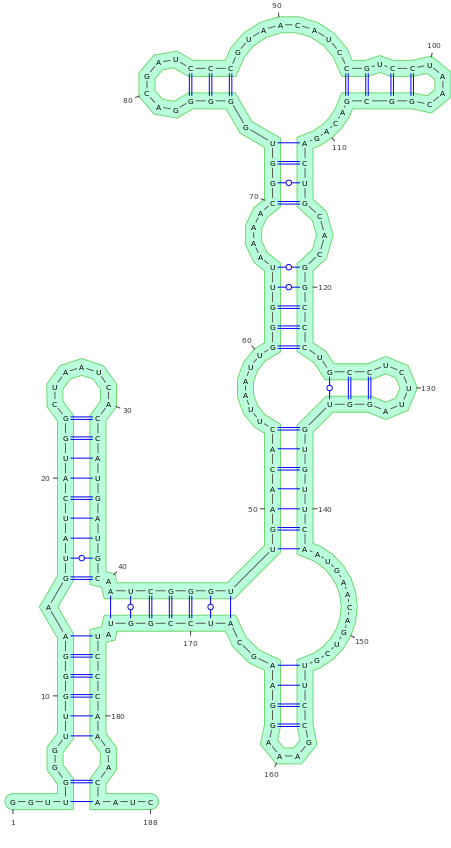
\includegraphics[width=.4\linewidth]{graphs/Supp_structures/1M7ILUMg_1M7ILU3Mg}\\}
\end{document}
